\chapter{Results}

\todo[inline]{fix the captions for the figures, see the article for the correct captions.}

\section{Results of the Baseline activity}
In the initial experiment, the baseline activity of the CA3 network was
observed from the \textit{original model} by
\textcite{sanjayImpairedDendriticInhibition2015}. The network was simulated for
5000 ms and showed somewhat synchronous activity throughout all three
populations (pyr, BC and OLM). Basket cells showed a higher firing rate
compared to the pyramidal cells and OLM cells. The basket cells seem to swap
between states of synchrony and asynchrony which is not observed in the other
two populations. The OLM cells showed a lower firing rate compared to the
pyramidal cells and basket cells. The baseline activity of the CA3 network is
shown in figure~\ref{fig:baseline_activity}.

\begin{figure}[htbp]
    \centering
    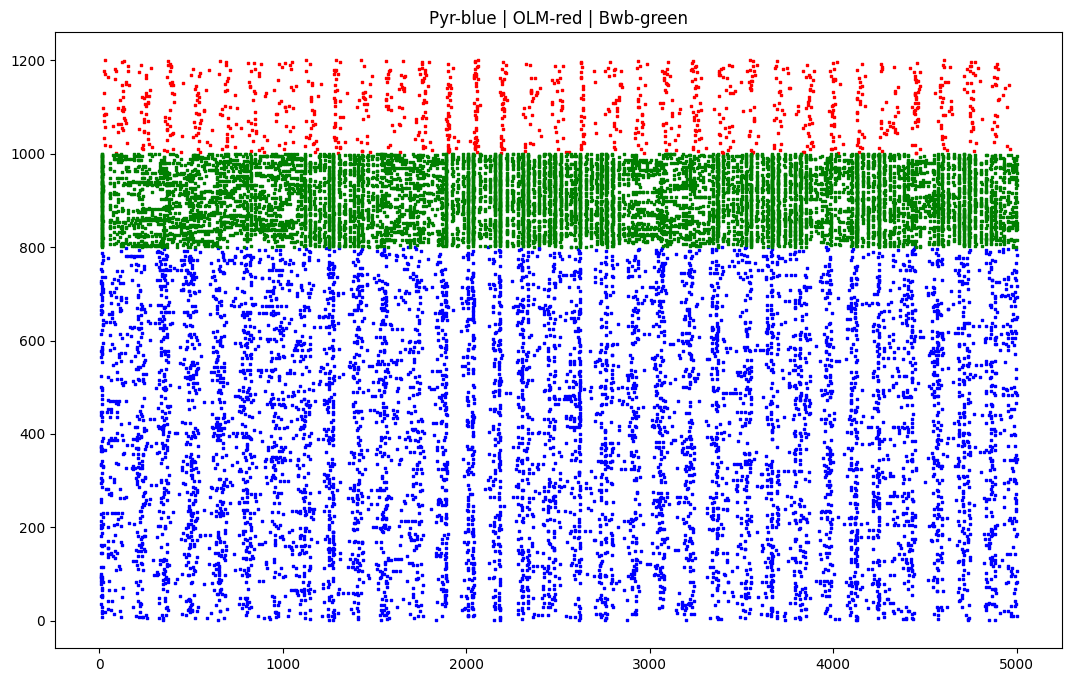
\includegraphics[width=0.9\textwidth]{Network_spike_activity_OLM_baseline.png}
    \caption[Baseline activity of the CA3 network]{Baseline activity of the CA3 network.}\label{fig:baseline_activity}
    \begin{minipage}{0.9\textwidth}
        The above figure shows the baseline activity of the CA3 network. The network was simulated for 5000 ms. The spike activity in time of the Pyr cells, BC cells, and OLM cells are shown based on the Neuron ID\@. ID 0--799 = Pyramidal (blue), 800--999 = BC (green), 1000--1200 = OLM (red). The x-axis represents the time in ms and the y-axis represents the neuron ID\@.
    \end{minipage}
\end{figure}

\section{Results of the Model validation}
To test whether our implementation of the CA3 network was able to replicate
more elaborate results, results from figure 6 of the original
\textcite{sanjayImpairedDendriticInhibition2015} article were replicated in
figure~\ref{fig:validation_firing_rates},~\ref{fig:validation_frequencies} and
~\ref{fig:validation_power}. The results show that the model was able to
replicate the results of the original article with slightly lower firing rates,
theta-gamma frequencies and power, which can be seen in
table~\ref{tab:validation_results}. The original article results are visible in
the methods section in table~\ref{tab:original_validation_results}.

\begin{figure}[htbp]
    \centering
    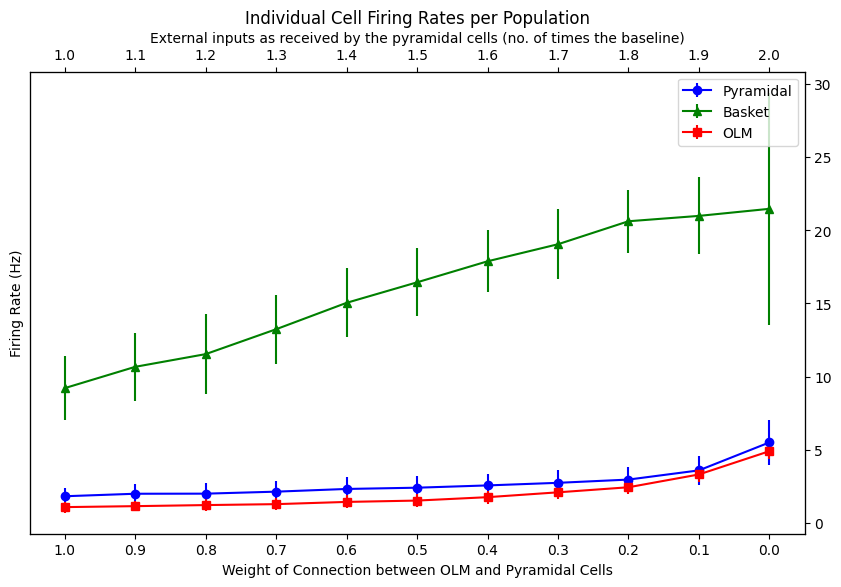
\includegraphics[width=0.9\textwidth]{Sanjay_validation_firing_rates.png}
    \caption[Validation of the firing rates]{Validation of the firing rates.}\label{fig:validation_firing_rates}
    \begin{minipage}{0.9\textwidth}
        The above figure shows the firing rates of the Pyr cells, BC cells, and OLM cells when dendritic inhibition is decreased and external noise is increased.
        The firing rates were calculated from the spike activity of the cells in each population for the duration of the simulation (5000 ms).
        The double x-axis represents both decrement in the weight of dendritic inhibition on pyramidal cells by OLM interneurons,
        while simultaneously increasing external noise stimulation to pyramidal cells.
        External noise levels rise and inhibition decreases by increments of 0.1, each representing a 10\% change relative to the baseline.
        The y-axis represents the firing rate in Hz.
        The firing rates are per cell type: Pyr (blue), Basket (green) and OLM (red).
        The error bars represent the standard deviation of the firing rates.
    \end{minipage}
\end{figure}

\begin{figure}[htbp]
    \centering
    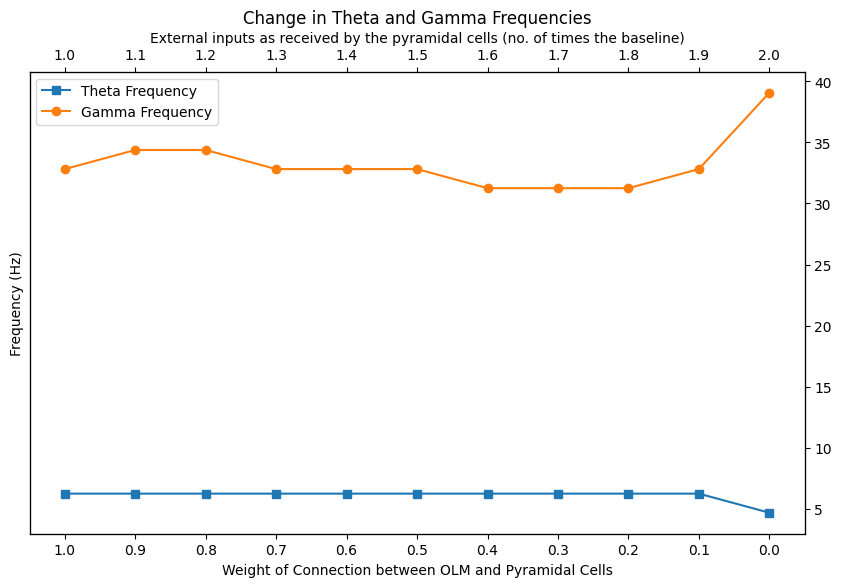
\includegraphics[width=0.9\textwidth]{Sanjay_validation_frequencies.png}
    \caption[Validation of the firing rates]{Validation of dominant frequencies.}\label{fig:validation_frequencies}
    \begin{minipage}{0.9\textwidth}
        The above figure shows the dominant theta-gamma frequencies in the network activity when dendritic inhibition is decreased and external noise is increased.
        The double x-axis represents both decrement in the weight of dendritic inhibition on pyramidal cells by OLM interneurons,
        while simultaneously increasing external noise stimulation to pyramidal cells.
        External noise levels rise and inhibition decreases by increments of 0.1, each representing a 10\% change relative to the baseline.
        The y-axis represents the dominant frequency in Hz for both theta (3--12 Hz, blue) and gamma (30--80 Hz, orange) oscillatory bands.
    \end{minipage}
\end{figure}

\begin{figure}[htbp]
    \centering
    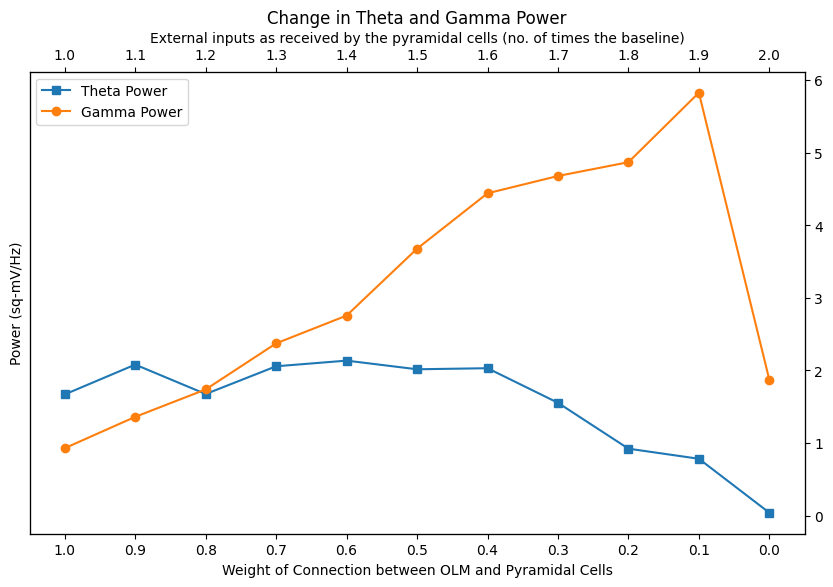
\includegraphics[width=0.9\textwidth]{Sanjay_validation_power.png}
    \caption[Validation of the firing rates]{Validation of Theta-Gamma power.}\label{fig:validation_power}
    \begin{minipage}{0.9\textwidth}
        The above figure shows the power of the theta and gamma oscillations in the network when dendritic inhibition is decreased and external noise is increased.
        The double x-axis represents both decrement in the weight of dendritic inhibition on pyramidal cells by OLM interneurons,
        while simultaneously increasing external noise stimulation to pyramidal cells.
        External noise levels rise and inhibition decreases by increments of 0.1, each representing a 10\% change relative to the baseline.
        The y-axis represents the theta and gamma power (blue and orange, respectively).
    \end{minipage}
\end{figure}

\begin{table}[htbp]
    \centering
    \caption[Summary of Model validation: Network simulation Parameters and Results]{Overview of Model Validation Network Simulation Settings and Outcomes.
        Variations in the firing rates of cell populations, alongside theta and gamma oscillations within the local field potential, as well as the alterations in their intensity upon the decrease of dendritic inhibition and the concurrent enhancement of external stimuli to the pyramidal neurons.}\label{tab:validation_results}
    \begin{adjustbox}{width=\textwidth}
        \begin{tabular}{ccccccccc}
            \hline
            OLM-Pyr Wt & External Wt & \CellWithForcedBreak{Pyr (Hz)                                                     \\ + Std} & \CellWithForcedBreak{BWB (Hz) \\ + Std} & \CellWithForcedBreak{OLM (Hz) \\ + Std} & \CellWithForcedBreak{Theta \\ Freq (Hz)} & \CellWithForcedBreak{Theta power \\ (mV\textsuperscript{2} Hz\textsuperscript{-1})} & \CellWithForcedBreak{Gamma \\ Freq (Hz)} & \CellWithForcedBreak{Gamma power \\ (mV\textsuperscript{2} Hz\textsuperscript{-1})} \\
            \hline
            1.0X       & 1.0X        & 1.83±0.58                     & 9.21±2.20  & 1.08±0.38 & 6.2 & 1.67 & 32.8 & 0.93 \\
            0.9X       & 1.1X        & 2.00±0.64                     & 10.67±2.31 & 1.15±0.36 & 6.2 & 2.08 & 34.4 & 1.36 \\
            0.8X       & 1.2X        & 2.00±0.71                     & 11.54±2.72 & 1.22±0.39 & 6.2 & 1.67 & 34.4 & 1.74 \\
            0.7X       & 1.3X        & 2.14±0.74                     & 13.24±2.36 & 1.29±0.42 & 6.2 & 2.06 & 32.8 & 2.37 \\
            0.6X       & 1.4X        & 2.33±0.79                     & 15.04±2.35 & 1.44±0.45 & 6.2 & 2.13 & 32.8 & 2.76 \\
            0.5X       & 1.5X        & 2.41±0.80                     & 16.44±2.31 & 1.53±0.45 & 6.2 & 2.02 & 32.8 & 3.68 \\
            0.4X       & 1.6X        & 2.57±0.79                     & 17.88±2.12 & 1.76±0.45 & 6.2 & 2.03 & 31.2 & 4.44 \\
            0.3X       & 1.7X        & 2.74±0.86                     & 19.04±2.38 & 2.10±0.49 & 6.2 & 1.55 & 31.2 & 4.68 \\
            0.2X       & 1.8X        & 2.97±0.88                     & 20.61±2.14 & 2.44±0.48 & 6.2 & 0.92 & 31.2 & 4.87 \\
            0.1X       & 1.9X        & 3.59±0.99                     & 20.98±2.62 & 3.31±0.50 & 6.2 & 0.78 & 32.8 & 5.82 \\
            0.0X       & 2.0X        & 5.50±1.52                     & 21.46±7.93 & 4.90±0.52 & 4.7 & 0.04 & 39.1 & 1.87 \\
            \hline
        \end{tabular}
    \end{adjustbox}
\end{table}
\pagebreak
\section{Results of the Sodium-Potassium variants}

\todo[inline]{add some text for the firing rates plot of sodium potassium}

\begin{figure}[htbp]
    \centering
    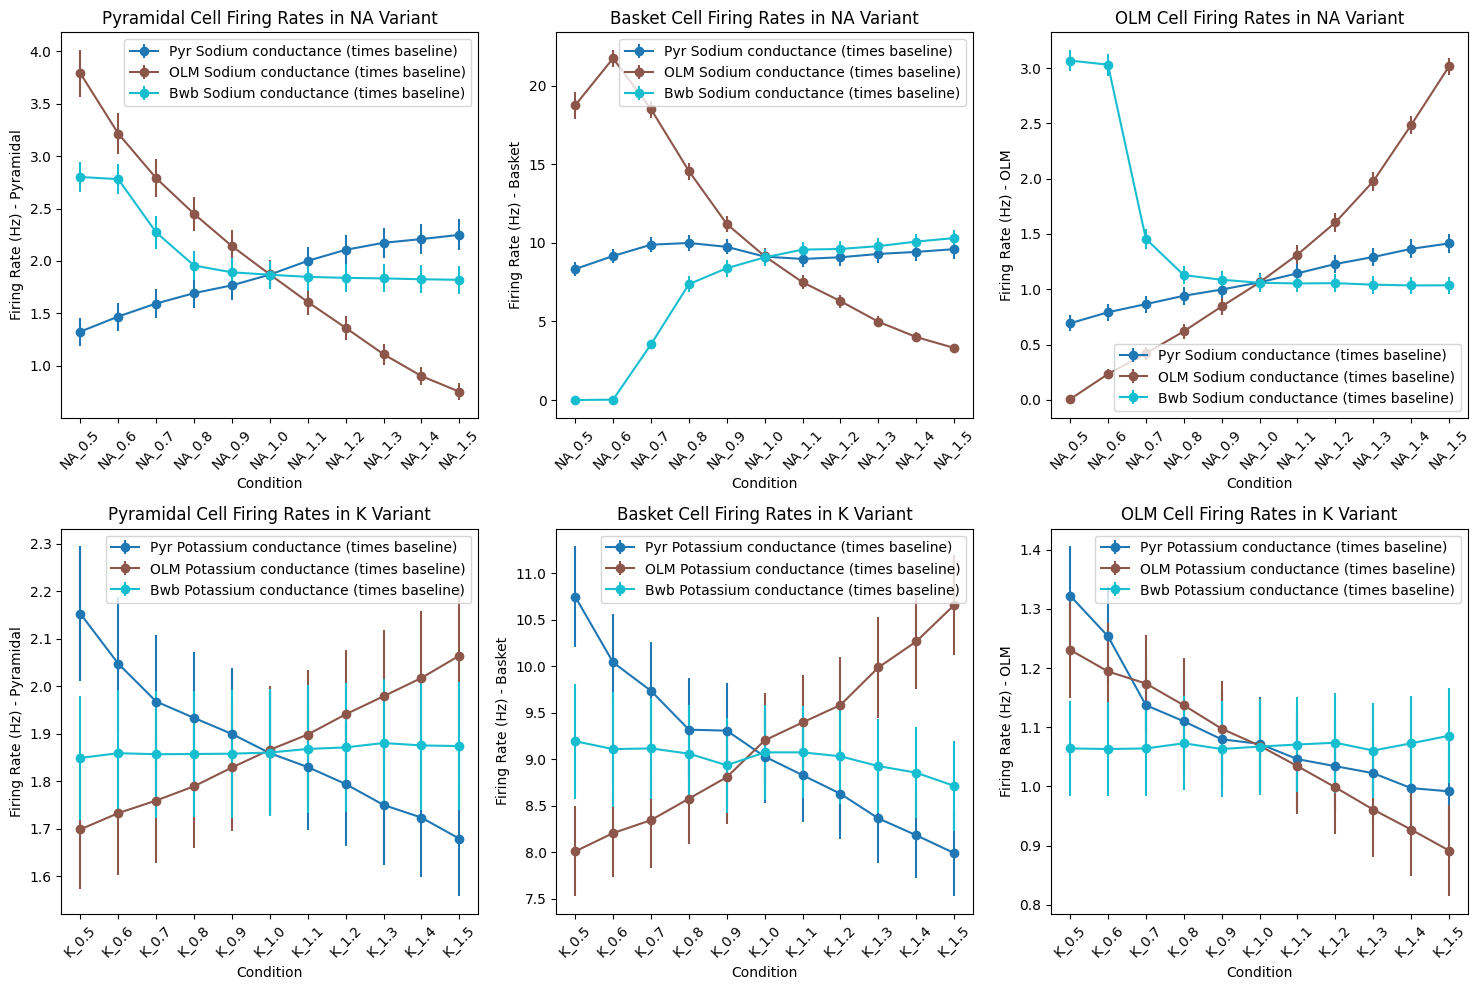
\includegraphics[width=1.0\textwidth]{Cell_firing_rates_per_pop_per_variant.png}
    \caption[Sodium-Potassium variants: Firing rates per population]{Sodium-Potassium variants: Firing rates per population.}\label{fig:sodium_potassium_firing_rates}
    \begin{minipage}{0.9\textwidth}
        The above figure shows the firing rates of the Pyr cells, BC cells, and OLM cells for each modified cell type.
        Each of the three cell types either had modified sodium or potassium conductance.
        The firing rates were calculated from the spike activity of the cells in each population for the duration of the simulation (5000 ms).
        The x-axis represents the percentage amount of changed sodium or potassium conductance, times the baseline.
        The y-axis represents the firing rate in Hz.
        The firing rates are per cell type: Pyr (blue), Basket (cyan) and OLM (red).
        The error bars represent the standard error of the mean (SEM) of the firing rates per population.
    \end{minipage}
\end{figure}

\begin{figure}[htbp]
    \centering
    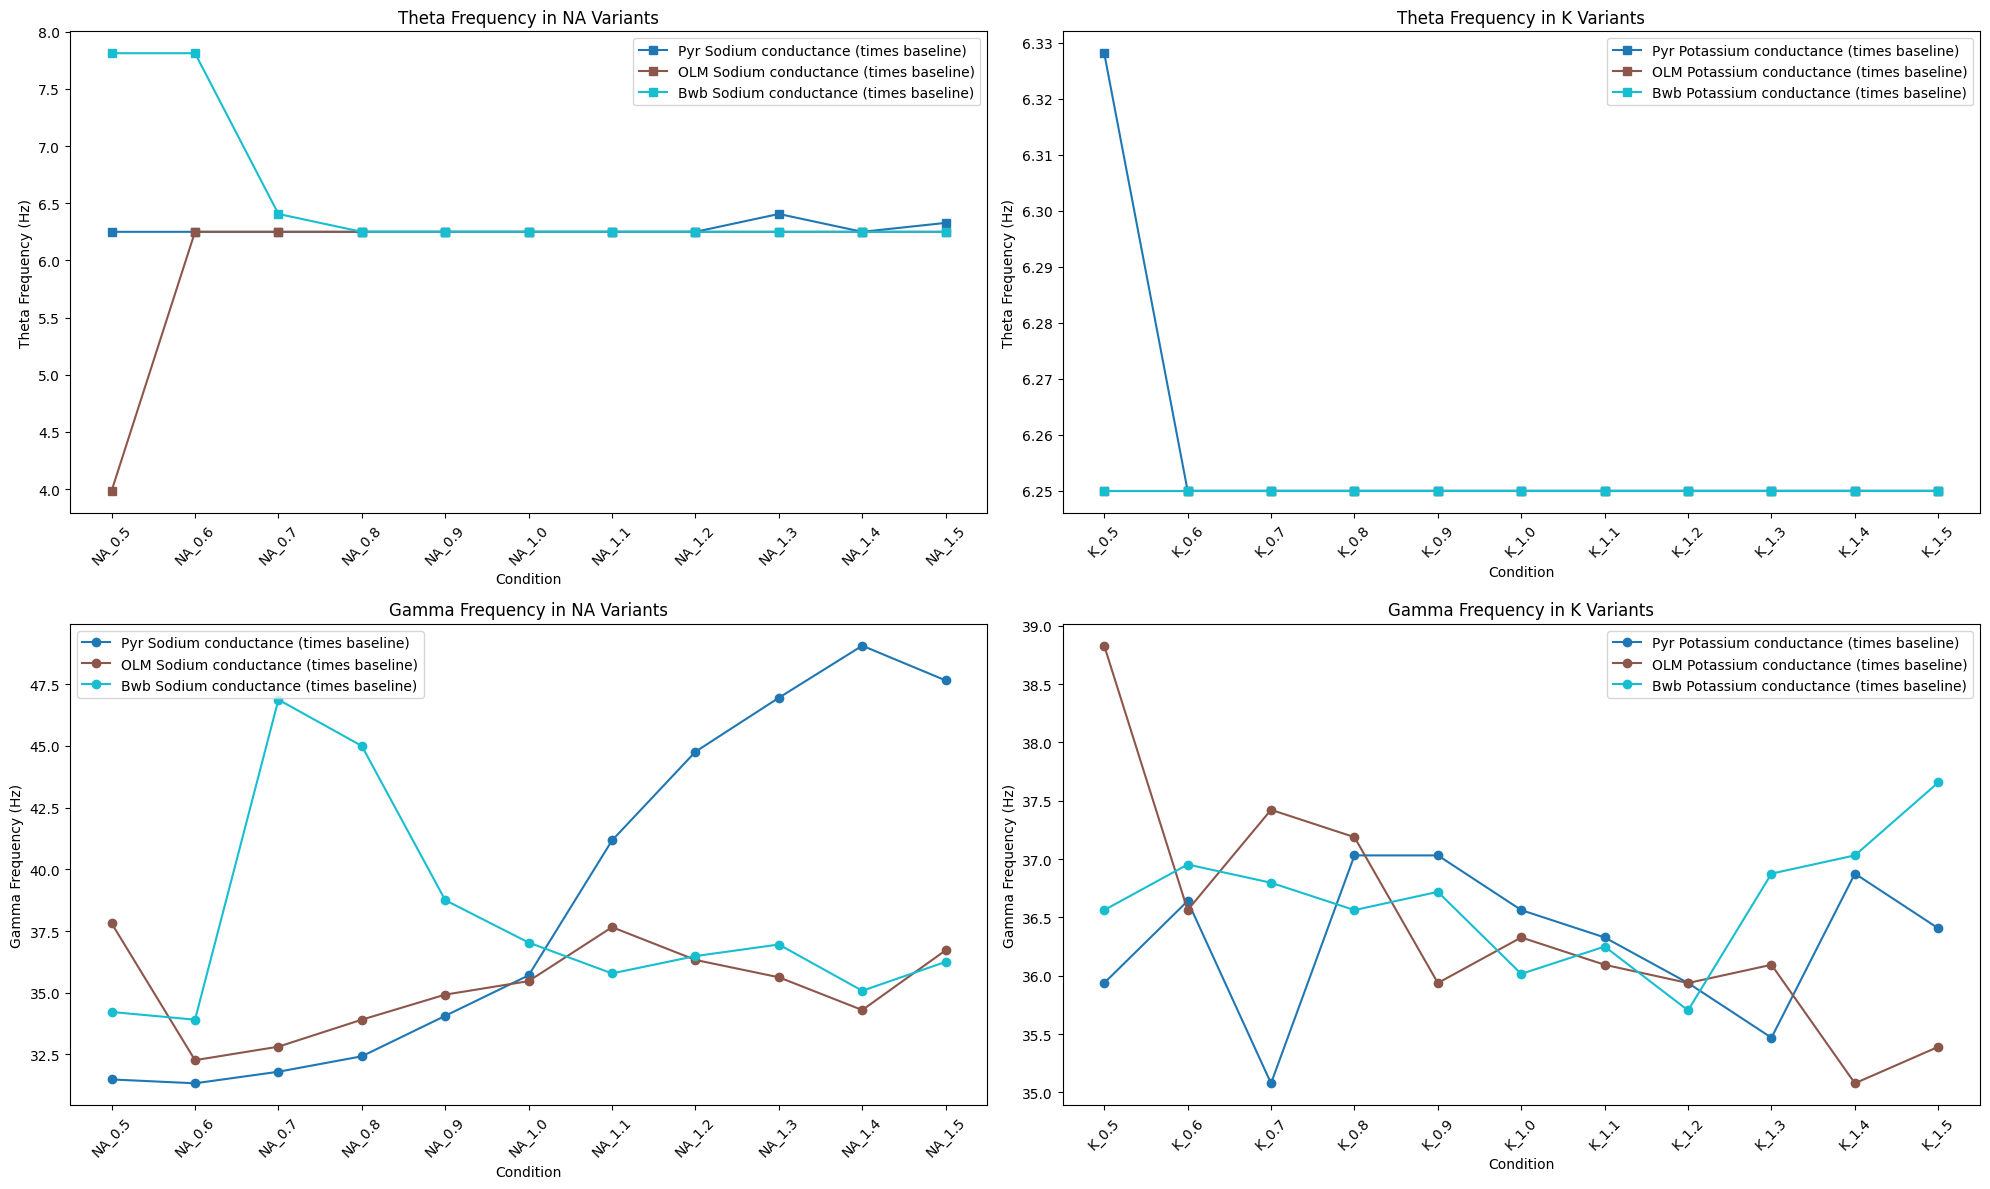
\includegraphics[width=1.0\textwidth]{Theta_gamma_freqs_variants.png}
    \caption[Sodium-Potassium variants: Dominant frequencies]{Sodium-Potassium variants: Dominant frequencies.}\label{fig:sodium_potassium_frequencies}
    \begin{minipage}{0.9\textwidth}
        The above figure shows the dominant theta-gamma frequencies in the network activity for each modified cell type.
        Each of the three cell types either had modified sodium or potassium conductance (pyr = blue, OLM = red, basket = cyan).
        The dominant frequencies were calculated from the local field potential (LFP) for the duration of the simulation (5000 ms).
        The x-axis represents the percentage amount of changed sodium or potassium conductance, times the baseline.
        The y-axis represents the dominant frequency in Hz for both theta (3--12 Hz, blue) and gamma (30--80 Hz, orange) oscillatory bands.
    \end{minipage}
\end{figure}
\begin{figure}[htbp]
    \centering
    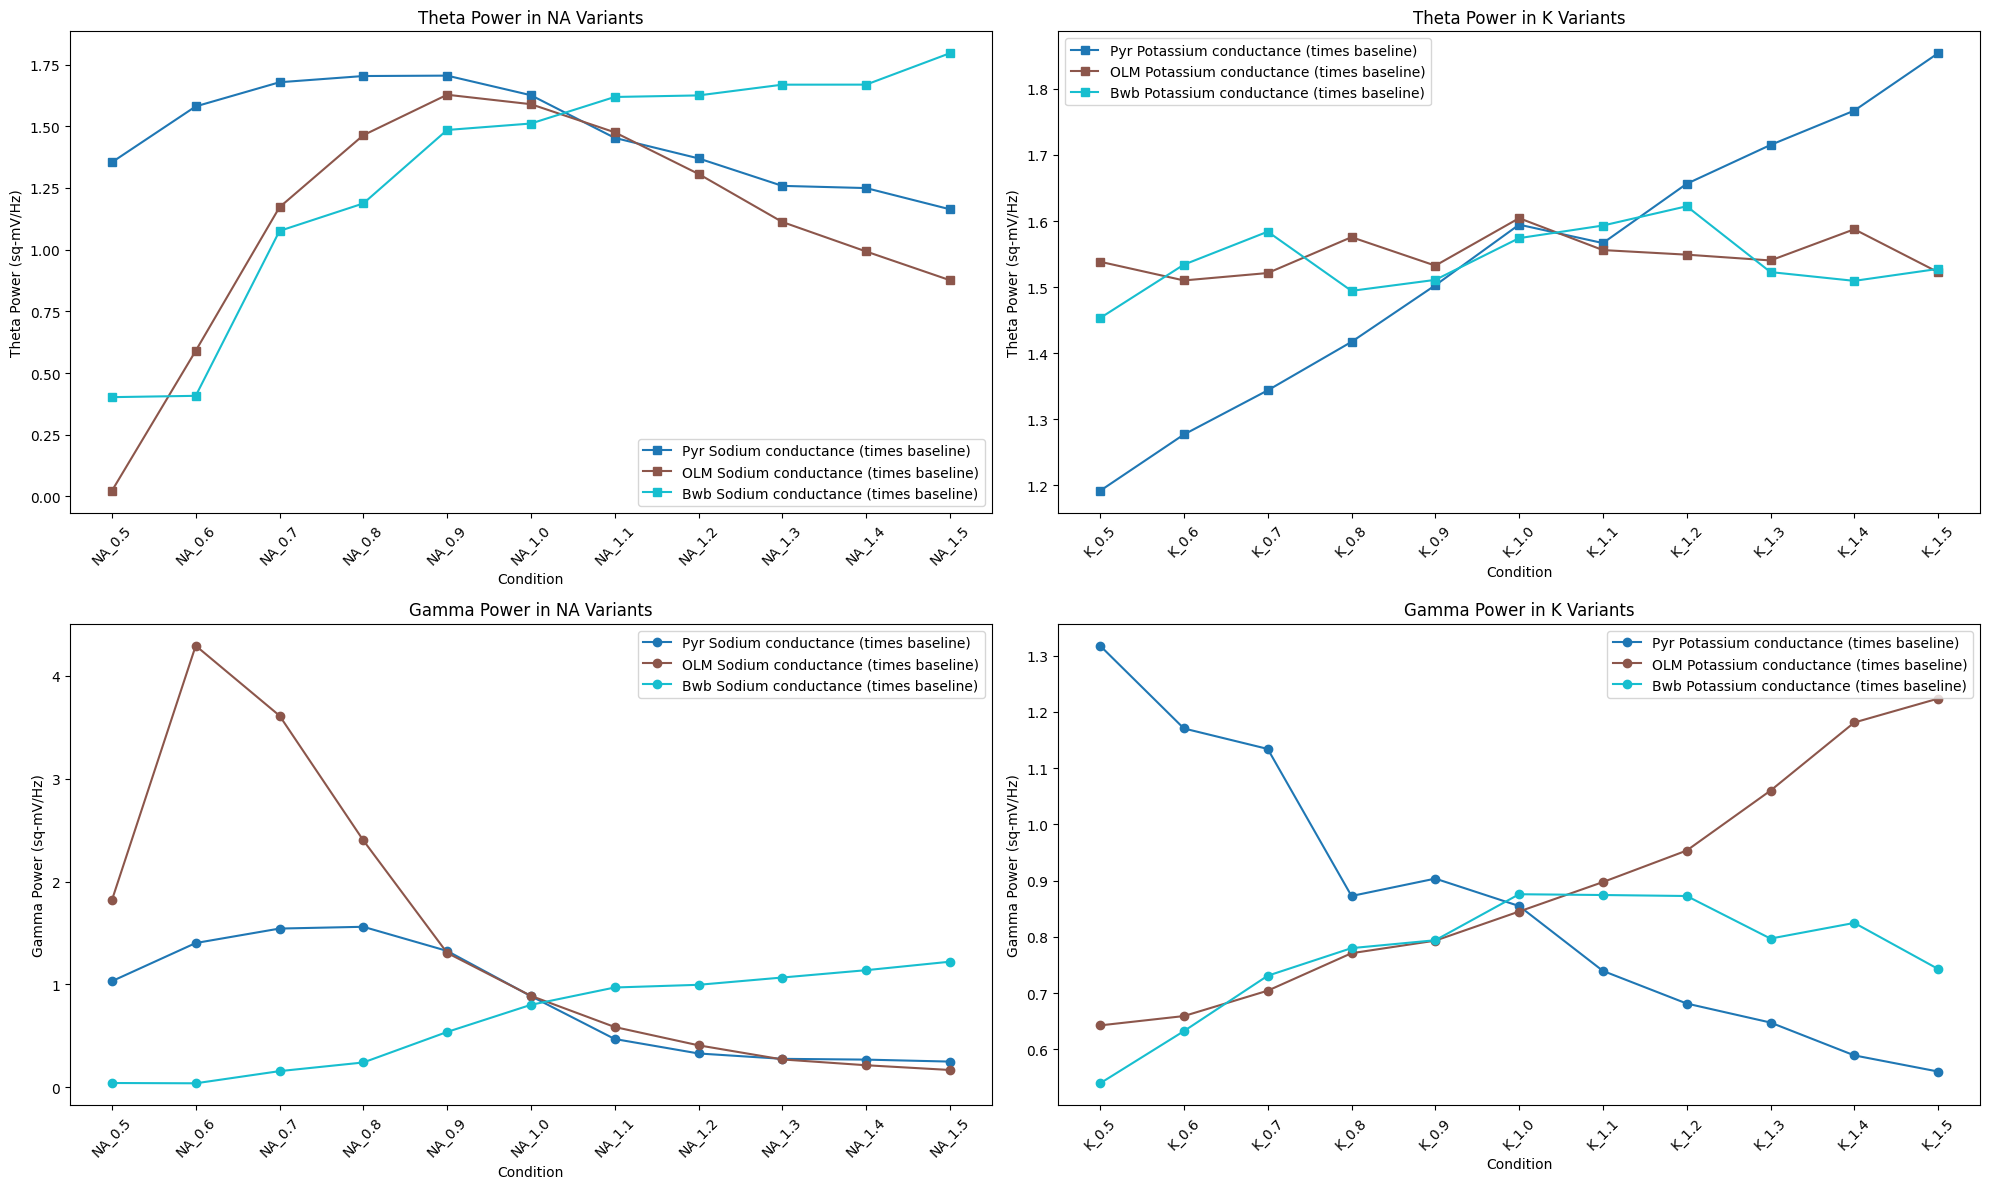
\includegraphics[width=1.0\textwidth]{Theta_gamma_power_variants.png}
    \caption[Sodium-Potassium variants: Theta-Gamma power]{Sodium-Potassium variants: Theta-Gamma power.}\label{fig:sodium_potassium_power}
    \begin{minipage}{0.9\textwidth}
        The above figure shows the power of the theta and gamma oscillations in the network for each modified cell type.
        Each of the three cell types either had modified sodium or potassium conductance (pyr = blue, OLM = red, basket = cyan).
        The power of the theta and gamma oscillations were calculated from the local field potential (LFP) for the duration of the simulation (5000 ms).
        The x-axis represents the percentage amount of changed sodium or potassium conductance, times the baseline.
        The y-axis represents the theta and gamma power (blue and orange, respectively).
    \end{minipage}
\end{figure}
\pagebreak

\section{Results of the External Noise variants}

\todo[inline]{don't forget to add some text to the previous results sections, not just captions under figures.}

\section{Results of the External Noise: Burst analysis}

\section{Results of the Recurrent Connections variants}
